\documentclass[a4paper,12pt]{article}

% ======================================================================
% PACKAGES
% ======================================================================
\usepackage[utf8]{inputenc}
\usepackage[T1]{fontenc}
\usepackage{amsmath,amssymb}
\usepackage{array}
\usepackage{booktabs}
\usepackage{geometry}
\usepackage{parskip}
\usepackage{enumitem}
\usepackage{caption}
\usepackage{hyperref}
\usepackage{tabularx}
\usepackage{xcolor}
\usepackage[most]{tcolorbox}
\usepackage{float}
\usepackage{siunitx}
\usepackage{graphicx}
\usepackage{tikz}
\usetikzlibrary{arrows.meta,positioning,shapes.geometric,calc}

\geometry{margin=2.5cm}

\hypersetup{
    colorlinks=true,
    linkcolor=blue!60!black,
    urlcolor=blue!60!black,
    citecolor=blue!60!black
}

\setlist[itemize]{topsep=3pt,itemsep=2pt,parsep=0pt}
\setlist[enumerate]{topsep=3pt,itemsep=2pt,parsep=0pt}
\captionsetup{font=small,labelfont=bf}

\newcolumntype{Y}{>{\raggedright\arraybackslash}X}

% ======================================================================
% BOX STYLES
% ======================================================================
\newtcolorbox{notebox}[1][]{
    enhanced,
    colback=blue!4!white,
    colframe=blue!55!black,
    fonttitle=\bfseries,
    title=#1,
    boxrule=0.6pt,
    arc=2mm,
    left=2mm,right=2mm,top=1mm,bottom=1mm
}

\newtcolorbox{warnbox}[1][]{
    enhanced,
    colback=orange!5!white,
    colframe=orange!65!black,
    fonttitle=\bfseries,
    title=#1,
    boxrule=0.6pt,
    arc=2mm,
    left=2mm,right=2mm,top=1mm,bottom=1mm
}

\newtcolorbox{keybox}[1][]{
    enhanced,
    colback=green!4!white,
    colframe=green!45!black,
    fonttitle=\bfseries,
    title=#1,
    boxrule=0.6pt,
    arc=2mm,
    left=2mm,right=2mm,top=1mm,bottom=1mm
}

\newtcolorbox{calcbox}[1][]{
    enhanced,
    colback=purple!4!white,
    colframe=purple!55!black,
    fonttitle=\bfseries,
    title=#1,
    boxrule=0.6pt,
    arc=2mm,
    left=2mm,right=2mm,top=1mm,bottom=1mm
}

\newtcolorbox{errbox}[1][]{
    enhanced,
    colback=red!4!white,
    colframe=red!60!black,
    fonttitle=\bfseries,
    title=#1,
    boxrule=0.6pt,
    arc=2mm,
    left=2mm,right=2mm,top=1mm,bottom=1mm
}

% ======================================================================
% TIKZ STYLES
% ======================================================================
\tikzset{
    workflowbox/.style={
        rectangle,
        rounded corners,
        draw=#1!70!black,
        fill=#1!8!white,
        thick,
        align=center,
        text width=2.75cm,
        minimum height=1.75cm,
        inner sep=4pt
    },
    smallworkflowbox/.style={
        rectangle,
        rounded corners,
        draw=#1!70!black,
        fill=#1!8!white,
        thick,
        align=center,
        text width=2.95cm,
        minimum height=1.55cm,
        inner sep=4pt
    },
    tinyworkflowbox/.style={
        rectangle,
        rounded corners,
        draw=#1!70!black,
        fill=#1!8!white,
        thick,
        align=center,
        text width=2.45cm,
        minimum height=1.45cm,
        inner sep=3pt
    },
    workflowarrow/.style={
        -{Latex[length=2mm]},
        thick,
        draw=black!65
    },
    feedbackarrow/.style={
        -{Latex[length=2mm]},
        thick,
        dashed,
        draw=black!55
    }
}

% ======================================================================
% TITLE
% ======================================================================
\title{\textbf{RSE3010: Mine Geotechnical Engineering}\\Week 2 Study Notes}
\author{Monash University, Semester 1, 2026}
\date{Based on Week 2 Lecture Slides}

\begin{document}

\maketitle

% ======================================================================
\section{Week 2: Intact Rock Mechanics -- Failure Criteria}
% ======================================================================

\subsection{Purpose}

To understand the fundamental failure criteria for intact rock, specifically the
Mohr--Coulomb and Hoek--Brown criteria, and to learn how to derive strength parameters
from laboratory data. This knowledge forms the basis for characterising intact rock
behaviour before considering rock mass structure.

\begin{keybox}[Core idea]
Week 2 is the first calculation-based step in the design chain:
\[
\text{Laboratory data} \rightarrow \text{Failure criterion} \rightarrow
\text{Strength parameters} \rightarrow \text{Design model}
\]
The parameters derived here are later used in rock mass classification, Hoek--Brown rock
mass parameter derivation, and numerical modelling.
\end{keybox}

% ======================================================================
\subsection{Learning Objectives}

By the end of this week, students should be able to:
\begin{itemize}
    \item review the concept of stress, strain, and principal stresses;
    \item understand gravitational and tectonic components of in-situ stress;
    \item distinguish between in-situ principal stresses and stresses used in failure criteria;
    \item understand the Mohr--Coulomb failure criterion and its limitations;
    \item apply the Hoek--Brown failure criterion for intact rock;
    \item estimate Mohr--Coulomb parameters \(c\) and \(\phi\) from Hoek--Brown using
    both the graphical Mohr circle method and the linear regression method; and
    \item determine tensile strength using the Hoek--Brown criterion and the tensile cut-off.
\end{itemize}

% ======================================================================
\section{Overview of Material Failure Theory}
% ======================================================================

Material failure theory describes how materials deform and ultimately fail under stress.
Different criteria are used depending on the material type, loading condition, stress
level, and purpose of analysis.

\begin{keybox}[Big picture]
No single failure criterion is universally correct. Each criterion is a simplified model
of reality, developed for particular material types and stress conditions. The engineer
must justify the selected criterion based on the project problem.
\end{keybox}

% ----------------------------------------------------------------------
\subsection{Categories of Failure Criteria}

\subsubsection{Phenomenological or Stress-Based Criteria}

These criteria define failure when stress reaches a critical condition.

\begin{table}[H]
\centering
\small
\begin{tabularx}{\textwidth}{l Y Y}
\toprule
\textbf{Criterion} & \textbf{Main idea} & \textbf{Typical use} \\
\midrule
Mohr--Coulomb & Linear cohesion--friction envelope & Soils, weak rocks, rock masses, design calculations, numerical modelling \\
Rankine & Maximum principal stress criterion & Brittle tensile failure and simple stress-limit checks \\
Tresca & Maximum shear stress criterion & Ductile metals under simple loading \\
von Mises & Distortional strain energy criterion & Ductile metals and plasticity models \\
Hoek--Brown & Nonlinear confinement-dependent rock strength & Intact rock and rock mass strength estimation \\
Drucker--Prager & Smooth pressure-dependent approximation of Mohr--Coulomb & Numerical modelling and plasticity formulations \\
Cam--Clay & Critical-state soil mechanics model & Normally consolidated clays and advanced soil modelling \\
\bottomrule
\end{tabularx}
\caption{Common phenomenological failure criteria.}
\end{table}

\begin{notebox}[Engineering relevance in this unit]
The main focus of RSE3010 is:
\begin{itemize}
    \item \textbf{Hoek--Brown}: used to represent nonlinear rock behaviour;
    \item \textbf{Mohr--Coulomb}: used as a practical design and numerical modelling form.
\end{itemize}
Most practical rock engineering workflows use Hoek--Brown to derive rock strength, then
convert to equivalent Mohr--Coulomb parameters when required by calculations or software.
\end{notebox}

% ----------------------------------------------------------------------
\subsubsection{Fracture Mechanics-Based Criteria}

These criteria focus on crack initiation and crack propagation rather than only the overall
stress state.

\begin{itemize}
    \item \textbf{Griffith theory}: failure occurs when sufficient energy is available for
    a crack to grow.
    \item This is especially relevant to brittle materials such as rock, concrete, and glass.
\end{itemize}

\begin{warnbox}[Key insight]
Rock is usually a pre-cracked material. Failure often initiates from micro-cracks,
bedding planes, joints, or other defects rather than from a perfectly homogeneous stress
state.
\end{warnbox}

% ----------------------------------------------------------------------
\subsubsection{Energy-Based Methods}

Energy-based methods are useful when stress-based approaches become insufficient, for
example:
\begin{itemize}
    \item anisotropic materials;
    \item complex loading paths;
    \item dynamic loading;
    \item fracture propagation; and
    \item advanced numerical modelling.
\end{itemize}

% ----------------------------------------------------------------------
\subsection{Material Failure Theory to Design Workflow}

Figure~\ref{fig:failure_workflow} summarises how failure theory is used in engineering
design.

\begin{figure}[H]
\centering
\resizebox{\textwidth}{!}{%
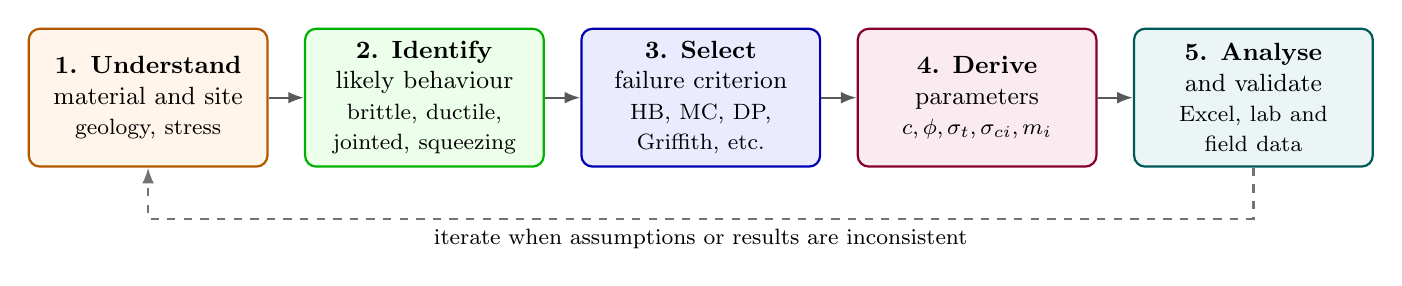
\begin{tikzpicture}[node distance=0.45cm, font=\small]

\node[workflowbox=orange] (step1)
{\textbf{1. Understand}\\ material and site\\
\footnotesize geology, stress};

\node[workflowbox=green, right=of step1] (step2)
{\textbf{2. Identify}\\ likely behaviour\\
\footnotesize brittle, ductile, jointed, squeezing};

\node[workflowbox=blue, right=of step2] (step3)
{\textbf{3. Select}\\ failure criterion\\
\footnotesize HB, MC, DP, Griffith, etc.};

\node[workflowbox=purple, right=of step3] (step4)
{\textbf{4. Derive}\\ parameters\\
\footnotesize \(c,\phi,\sigma_t,\sigma_{ci},m_i\)};

\node[workflowbox=teal, right=of step4] (step5)
{\textbf{5. Analyse}\\ and validate\\
\footnotesize Excel, lab and field data};

\draw[workflowarrow] (step1) -- (step2);
\draw[workflowarrow] (step2) -- (step3);
\draw[workflowarrow] (step3) -- (step4);
\draw[workflowarrow] (step4) -- (step5);

\draw[feedbackarrow] (step5.south) -- ++(0,-0.65) -| node[pos=0.25,below,font=\footnotesize]
{iterate when assumptions or results are inconsistent} (step1.south);

\end{tikzpicture}
}
\caption{Material failure theory to engineering design workflow.}
\label{fig:failure_workflow}
\end{figure}

\begin{keybox}[Connection to Week 2]
Week 2 focuses on the middle of the workflow: selecting suitable intact-rock failure
criteria and deriving parameters from laboratory data. Weeks 3--4 extend the same logic
from intact rock to jointed rock masses.
\end{keybox}

% ======================================================================
\section{How to Select the Appropriate Failure Criterion for a Project}
% ======================================================================

The failure criterion should be selected based on the engineering problem, not by
convenience alone. Table~\ref{tab:criterion_selection} gives a practical selection guide.

\begin{table}[H]
\centering
\footnotesize
\begin{tabularx}{\textwidth}{l Y Y Y}
\toprule
\textbf{Consideration} & \textbf{Key question} & \textbf{Recommended criterion} & \textbf{Typical use in this unit} \\
\midrule
Material type
& Is the material soil, intact rock, jointed rock, or concrete?
& Rock: HB/MC; soil: MC/DP/Cam--Clay; concrete: MC or fracture-based checks
& Rock projects use HB first, then MC when required. \\

Scale
& Are we analysing intact laboratory samples or tunnel-scale rock masses?
& Intact scale: intact HB; rock mass scale: generalised HB or equivalent MC
& Week 2 uses intact HB. Week 4 uses generalised HB for rock masses. \\

Confining stress
& Is confinement low, moderate, or high?
& Low confinement: MC may be adequate; high confinement: HB preferred
& Deep tunnels and caverns need HB sensitivity checks. \\

Failure mechanism
& Is failure brittle, shear-dominated, structurally controlled, or squeezing?
& Brittle: HB/Griffith concepts; shear: MC; structurally controlled: discontinuity and empirical methods
& Week 6 uses failure mechanism identification before support design. \\

Available data
& Do we have laboratory strength, GSI, RMR/Q, or only limited description?
& Detailed data: HB or advanced models; limited data: MC or empirical correlations
& Assignment 1 uses lab data, then classification, then design parameters. \\

Software requirement
& What model does the software require?
& RS2 commonly uses MC or HB; some analytical solutions require MC
& Use MC where specified, but justify how it was derived. \\

Purpose
& Is the purpose preliminary screening, parameter derivation, or final design?
& Preliminary: MC/empirical; parameter derivation: HB; detailed design: calibrated numerical model
& Week 2 derives parameters; later weeks compare empirical, analytical, and numerical methods. \\
\bottomrule
\end{tabularx}
\caption{Practical guide for selecting a failure criterion.}
\label{tab:criterion_selection}
\end{table}

\begin{warnbox}[Do not select criteria mechanically]
A common mistake is to say ``Mohr--Coulomb is used because it is simple''. A stronger
engineering justification is: ``Mohr--Coulomb is adopted because the analysis requires an
equivalent linear strength envelope over the project-relevant confinement range, and the
parameters are derived from Hoek--Brown using the in-situ stress range.''
\end{warnbox}

\subsection{Recommended Criterion Selection for Assignment 1}

For Assignment 1, the recommended logic is:

\begin{enumerate}
    \item \textbf{Week 2 -- Intact rock behaviour:}
    use the intact Hoek--Brown criterion to calculate confined compressive strength and
    tensile strength from \(\sigma_{ci}\) and \(m_i\).
    
    \item \textbf{Week 2 -- Equivalent design parameters:}
    convert Hoek--Brown to equivalent Mohr--Coulomb parameters \(c\) and \(\phi\) over
    the project-specific stress range \(0 \leq \sigma_3 \leq \sigma_{3,\mathrm{fit,max}}\).
    
    \item \textbf{Week 3 -- Rock mass quality:}
    use RMR, Q, and GSI to describe rock mass condition.
    
    \item \textbf{Week 4 -- Rock mass strength:}
    use the generalised Hoek--Brown criterion with GSI and disturbance factor \(D\), then
    convert to equivalent Mohr--Coulomb parameters for design calculations.
\end{enumerate}

\begin{keybox}[Practical selection for this project]
For the different rock types:
\[
\text{Intact rock strength: Hoek--Brown}
\quad \rightarrow \quad
\text{Design parameters: Mohr--Coulomb}
\]
This is the most defensible workflow because HB captures nonlinear rock behaviour, while
MC provides the \(c\) and \(\phi\) parameters required by many design calculations.
\end{keybox}

% ======================================================================
\section{Concept of Stress and Principal Stresses}
% ======================================================================

\subsection{Stress at a Point}

Stress describes the internal force intensity acting inside a material. At a point in a
three-dimensional body, stresses may act normal to a plane or tangential to a plane.

\begin{itemize}
    \item \textbf{Normal stress} acts perpendicular to a plane.
    \item \textbf{Shear stress} acts tangential to a plane.
\end{itemize}

In the general three-dimensional case, the stress state is represented by the stress tensor:
\[
\boldsymbol{\sigma}
=
\begin{bmatrix}
\sigma_{xx} & \tau_{xy} & \tau_{xz} \\
\tau_{yx} & \sigma_{yy} & \tau_{yz} \\
\tau_{zx} & \tau_{zy} & \sigma_{zz}
\end{bmatrix}
\]

\begin{notebox}[Conceptual meaning]
The stress tensor describes stress on the original coordinate planes. However, these
planes are not necessarily the planes on which shear stress is zero. By rotating the
coordinate system, we can find three mutually perpendicular planes where shear stress is
zero. The normal stresses on these planes are called the principal stresses.
\end{notebox}

\subsection{Principal Stresses}

The principal stresses are denoted by:
\[
\sigma_1,\quad \sigma_2,\quad \sigma_3
\]
with:
\[
\sigma_1 \geq \sigma_2 \geq \sigma_3
\]

where:
\begin{itemize}
    \item \(\sigma_1\) = maximum principal stress;
    \item \(\sigma_2\) = intermediate principal stress;
    \item \(\sigma_3\) = minimum principal stress.
\end{itemize}

\begin{keybox}[Sign convention]
In rock mechanics and in this unit, compressive stress is usually taken as positive.
Therefore, \(\sigma_1\) is the largest compressive principal stress and \(\sigma_3\) is the
smallest compressive principal stress.
\end{keybox}

% ======================================================================
\section{In-Situ Stress: Gravitational and Tectonic Components}
% ======================================================================

\subsection{What Is In-Situ Stress?}

In-situ stress is the natural stress existing in the ground before excavation. It is generated
by:
\begin{itemize}
    \item the weight of overlying rock or soil;
    \item tectonic plate movements;
    \item geological history, erosion, uplift, and residual stresses; and
    \item local geological structures such as faults, folds, and bedding.
\end{itemize}

\begin{warnbox}[Why students often find this difficult]
In-situ stress is not simply ``vertical stress plus horizontal stress''. It is a
three-dimensional stress state. The vertical stress is usually estimated from overburden,
but the horizontal stresses can be strongly affected by tectonic history and may be larger
than the vertical stress.
\end{warnbox}

\subsection{Vertical Stress from Overburden}

The vertical stress is commonly estimated as:
\[
\sigma_v = \gamma z
\]
where:
\begin{itemize}
    \item \(\sigma_v\) = vertical stress;
    \item \(\gamma\) = unit weight of overlying material;
    \item \(z\) = depth below ground surface.
\end{itemize}

For Assignment 1:
\[
\gamma = 27~\text{kN/m}^3 = 0.027~\text{MPa/m}
\]

Therefore:
\[
\sigma_v = 0.027z
\]

For example, at \(z=2000~\text{m}\):
\[
\sigma_v = 0.027 \times 2000 = 54~\text{MPa}
\]

\subsection{Horizontal Stresses}

The horizontal stresses are commonly expressed using in-situ stress ratios:
\[
\sigma_H = K_H \sigma_v
\]
\[
\sigma_h = K_h \sigma_v
\]

where:
\begin{itemize}
    \item \(\sigma_H\) = maximum horizontal stress;
    \item \(\sigma_h\) = minimum horizontal stress;
    \item \(K_H\) = maximum horizontal stress ratio;
    \item \(K_h\) = minimum horizontal stress ratio.
\end{itemize}

\begin{notebox}[Notation]
Use uppercase \(H\) for the maximum horizontal stress and lowercase \(h\) for the
minimum horizontal stress:
\[
\sigma_H \geq \sigma_h
\]
This avoids confusion with the vertical stress \(\sigma_v\).
\end{notebox}

\subsection{Elastic At-Rest Approximation}

If the ground is assumed to deform elastically under one-dimensional gravitational loading
with no lateral strain, the horizontal-to-vertical stress ratio may be estimated as:
\[
K_0 = \frac{\nu}{1-\nu}
\]

For example, if \(\nu = 0.25\):
\[
K_0 = \frac{0.25}{1-0.25} = 0.33
\]

\begin{warnbox}[Do not overuse \(K_0=\nu/(1-\nu)\)]
This equation is only a simple elastic approximation. It does not capture tectonic stress,
stress history, erosion, faulting, or locked-in residual stresses. In rock engineering,
measured or project-specific stress ratios are usually preferred where available.
\end{warnbox}

\subsection{Stress Regimes}

Depending on the relative magnitudes of \(\sigma_v\), \(\sigma_H\), and \(\sigma_h\), the
in-situ stress state may correspond to different tectonic regimes.

\begin{table}[H]
\centering
\small
\begin{tabularx}{\textwidth}{l c Y}
\toprule
\textbf{Stress regime} & \textbf{Principal stress order} & \textbf{Typical interpretation} \\
\midrule
Normal faulting &
\(\sigma_v = \sigma_1 > \sigma_H = \sigma_2 > \sigma_h = \sigma_3\) &
Vertical stress is the largest stress; common in extensional settings. \\
\midrule
Strike-slip faulting &
\(\sigma_H = \sigma_1 > \sigma_v = \sigma_2 > \sigma_h = \sigma_3\) &
Maximum horizontal stress is largest; vertical stress is intermediate. \\
\midrule
Reverse faulting &
\(\sigma_H = \sigma_1 > \sigma_h = \sigma_2 > \sigma_v = \sigma_3\) &
Both horizontal stresses exceed vertical stress; common in compressional settings. \\
\bottomrule
\end{tabularx}
\caption{Common stress regimes in rock mechanics.}
\end{table}

\begin{keybox}[Engineering implication]
The maximum principal stress may be vertical or horizontal. Therefore, do not assume
\(\sigma_1=\sigma_v\). First calculate or estimate \(\sigma_v\), \(\sigma_H\), and \(\sigma_h\),
then rank them to identify \(\sigma_1\), \(\sigma_2\), and \(\sigma_3\).
\end{keybox}

% ======================================================================
\section{Visual Workflow: From In-Situ Stress to Failure Criterion}
% ======================================================================

The following workflow helps connect field stress, principal stresses, and failure criteria.

\begin{figure}[H]
\centering
\resizebox{\textwidth}{!}{%
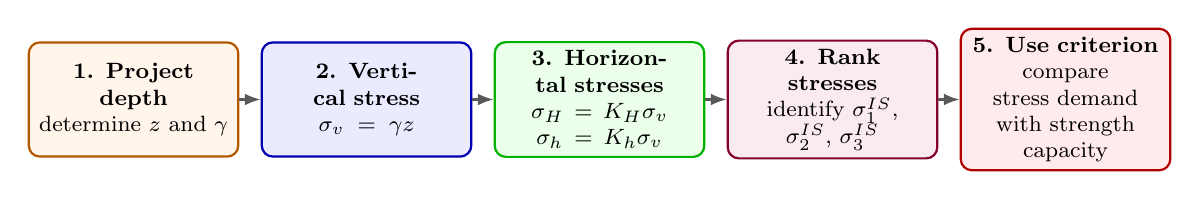
\begin{tikzpicture}[node distance=0.27cm, font=\footnotesize]

\node[tinyworkflowbox=orange] (a)
{\textbf{1. Project depth}\\
determine \(z\) and \(\gamma\)};

\node[tinyworkflowbox=blue, right=of a] (b)
{\textbf{2. Vertical stress}\\
\(\sigma_v=\gamma z\)};

\node[tinyworkflowbox=green, right=of b] (c)
{\textbf{3. Horizontal stresses}\\
\(\sigma_H=K_H\sigma_v\)\\
\(\sigma_h=K_h\sigma_v\)};

\node[tinyworkflowbox=purple, right=of c] (d)
{\textbf{4. Rank stresses}\\
identify \(\sigma_1^{IS}\), \(\sigma_2^{IS}\), \(\sigma_3^{IS}\)};

\node[tinyworkflowbox=red, right=of d] (e)
{\textbf{5. Use criterion}\\
compare stress demand\\
with strength capacity};

\draw[workflowarrow] (a) -- (b);
\draw[workflowarrow] (b) -- (c);
\draw[workflowarrow] (c) -- (d);
\draw[workflowarrow] (d) -- (e);

\end{tikzpicture}
}
\caption{Workflow for converting project depth and stress ratios into principal stresses for failure assessment.}
\label{fig:insitu_stress_workflow}
\end{figure}

% ======================================================================
\section{Avoiding Confusion: In-Situ Principal Stresses vs Hoek--Brown Stresses}
% ======================================================================

A common source of confusion is that the symbols \(\sigma_1\) and \(\sigma_3\) are used
in two related but different ways.

\subsection{In-Situ Principal Stresses}

In the in-situ stress context:
\[
\sigma_1^{IS},\quad \sigma_2^{IS},\quad \sigma_3^{IS}
\]
represent the current principal stresses already acting in the ground before excavation.

They are obtained by ranking:
\[
\sigma_v,\quad \sigma_H,\quad \sigma_h
\]

For example:
\[
\sigma_1^{IS} = \max(\sigma_v,\sigma_H,\sigma_h)
\]
\[
\sigma_3^{IS} = \min(\sigma_v,\sigma_H,\sigma_h)
\]

These are the \textbf{stress demand} imposed by the ground environment.

\subsection{Hoek--Brown Failure Stresses}

In the Hoek--Brown criterion:
\[
\sigma_1 =
\sigma_3 + \sigma_{ci}
\left(
m_i\frac{\sigma_3}{\sigma_{ci}} + 1
\right)^{1/2}
\]

\(\sigma_3\) is the confining stress applied to the specimen or rock mass, and
\(\sigma_1\) is the major principal stress at failure.

These are not automatically the same as the current in-situ stresses. Instead, the
Hoek--Brown equation describes the \textbf{strength capacity} of the material.

\begin{keybox}[Demand vs capacity]
\[
\text{In-situ stresses} = \textbf{stress demand}
\]
\[
\text{Hoek--Brown failure envelope} = \textbf{strength capacity}
\]
Failure is assessed by comparing demand with capacity.
\end{keybox}

\subsection{Recommended Notation to Avoid Confusion}

Use the following notation in teaching notes and worked examples:

\begin{table}[H]
\centering
\small
\begin{tabularx}{\textwidth}{l l Y}
\toprule
\textbf{Symbol} & \textbf{Meaning} & \textbf{Use} \\
\midrule
\(\sigma_v\) & Vertical in-situ stress & Calculated from \(\gamma z\). \\
\(\sigma_H\) & Maximum horizontal in-situ stress & Calculated from \(K_H\sigma_v\). \\
\(\sigma_h\) & Minimum horizontal in-situ stress & Calculated from \(K_h\sigma_v\). \\
\(\sigma_1^{IS}\) & Maximum in-situ principal stress & Current stress demand in the ground. \\
\(\sigma_3^{IS}\) & Minimum in-situ principal stress & Current minimum confinement in the ground. \\
\(\sigma_3\) in HB & Confining stress used in the failure criterion & Input variable for the HB strength envelope. \\
\(\sigma_1^f\) in HB & Major principal stress at failure & Strength capacity predicted by HB. \\
\(\sigma_{3,\mathrm{fit,max}}\) & Upper confining stress used for HB--MC fitting & Modelling choice used to define the regression range. \\
\bottomrule
\end{tabularx}
\caption{Recommended notation for distinguishing in-situ stresses and failure-criterion stresses.}
\end{table}

\begin{warnbox}[Most important distinction]
When using Hoek--Brown:
\[
\sigma_1^f \neq \sigma_1^{IS}
\]
in general.

\(\sigma_1^{IS}\) is the current maximum stress in the ground.  
\(\sigma_1^f\) is the stress required to cause failure at a given confinement.
\end{warnbox}

\subsection{How to Choose \(\sigma_{3,\mathrm{fit,max}}\)}

The value \(\sigma_{3,\mathrm{fit,max}}\) is not the minimum in-situ principal stress.
It is the upper limit of the confining stress range used to fit the nonlinear
Hoek--Brown envelope with an equivalent linear Mohr--Coulomb envelope.

\begin{notebox}[Recommended rule for this assignment]
For this assignment, use the simplified project-stress range:
\[
0 \leq \sigma_3 \leq \sigma_{3,\mathrm{fit,max}}
\]
where:
\[
\sigma_{3,\mathrm{fit,max}}=\max(\sigma_v,\sigma_{h,K})
\]

This convention gives a fitting range that covers the main project stress level in the
simplified two-stress calculation. The actual minimum in-situ principal stress is still:
\[
\sigma_3^{IS}=\min(\sigma_v,\sigma_{h,K})
\]
\end{notebox}

\begin{keybox}[Simple distinction]
\[
\sigma_3^{IS}=\text{minimum in-situ principal stress}
\]
\[
\sigma_{3,\mathrm{fit,max}}=\text{upper fitting limit for HB--MC conversion}
\]
The first is a real stress state in the ground. The second is a modelling choice for
curve fitting.
\end{keybox}

\begin{warnbox}[Why not always use \(\sigma_3^{IS}\) as the fitting limit?]
Using \(\sigma_3^{IS}\) as the upper fitting limit is possible, but it gives a narrower
fitting range. A narrower range usually gives higher \(\phi\) and lower \(c\), while a
wider range gives lower \(\phi\) and higher \(c\). Therefore, students must always state
the fitting range and justify it.
\end{warnbox}

\subsection{How This Applies to Assignment 1}

For Assignment 1, students should follow this logic:

\begin{enumerate}
    \item Calculate:
    \[
    \sigma_v = \gamma z
    \]
    
    \item Calculate the horizontal stress using the provided stress ratio:
    \[
    \sigma_{h,K} = K\sigma_v
    \]
    where \(\sigma_{h,K}\) is the project-specified horizontal stress used in the simplified
    two-dimensional calculation.
    
    \item Rank the stresses to identify the simplified in-situ principal stresses:
    \[
    \sigma_1^{IS} = \max(\sigma_v,\sigma_{h,K})
    \]
    \[
    \sigma_3^{IS} = \min(\sigma_v,\sigma_{h,K})
    \]
    
    \item For the Week 2 intact rock calculation under a fixed confining pressure, use:
    \[
    \sigma_3 = 20~\text{MPa}
    \]
    in the Hoek--Brown equation.
    
    \item For Mohr--Coulomb conversion, generate Hoek--Brown data over the selected
    fitting range:
    \[
    0 \leq \sigma_3 \leq \sigma_{3,\mathrm{fit,max}}
    \]
    where, for this assignment:
    \[
    \sigma_{3,\mathrm{fit,max}}=\max(\sigma_v,\sigma_{h,K})
    \]
    
    \item Clearly state the chosen fitting range and explain why it is relevant to the
    project stress condition.
\end{enumerate}

\begin{notebox}[Suggested wording for student reports]
``The in-situ stresses were first calculated from depth and stress ratio to define the
project stress condition. These stresses represent the stress demand. The Hoek--Brown
criterion was then used to estimate the intact rock strength capacity. Equivalent
Mohr--Coulomb parameters were obtained by fitting the Hoek--Brown envelope over the
project-relevant confinement range.''
\end{notebox}

% ======================================================================
\section{Mohr--Coulomb Failure Criterion}
% ======================================================================

\subsection{Basic Equation}

The Mohr--Coulomb criterion expresses shear strength \(\tau\) as a linear function of
normal stress \(\sigma_n\):
\[
\tau = c + \sigma_n \tan\phi
\]
where:
\begin{itemize}
    \item \(c\) = cohesion;
    \item \(\phi\) = friction angle;
    \item \(\sigma_n\) = normal stress on the failure plane.
\end{itemize}

In terms of principal stresses \((\sigma_1 \geq \sigma_2 \geq \sigma_3)\), failure occurs when:
\[
\sigma_1 =
\frac{2c\cos\phi + \sigma_3(1+\sin\phi)}
{1-\sin\phi}
\]

This can also be written as:
\[
\sigma_1 = \sigma_c + \sigma_3 \tan\psi
\]
where:
\[
\sigma_c =
\frac{2c\cos\phi}{1-\sin\phi},
\qquad
\tan\psi =
\frac{1+\sin\phi}{1-\sin\phi}
\]

\begin{calcbox}[Engineering interpretation]
The parameter \(c\) mainly controls strength at low confinement, while \(\phi\) controls
how rapidly strength increases with confining stress.
\end{calcbox}

% ----------------------------------------------------------------------
\subsection{Uniaxial and Tensile Strengths}

For \(\sigma_3 = 0\), the uniaxial compressive strength predicted by Mohr--Coulomb is:
\[
\sigma_c =
\frac{2c\cos\phi}{1-\sin\phi}
\]

For \(\sigma_1 = 0\), the uniaxial tensile strength is:
\[
\sigma_t =
-\frac{2c\cos\phi}{1+\sin\phi}
=
-\frac{\sigma_c(1-\sin\phi)}{1+\sin\phi}
\]

% ----------------------------------------------------------------------
\subsection{Orientation of Failure Plane}

The angle \(\theta\) between the failure plane and the direction of \(\sigma_1\) is:
\[
\theta = 45^\circ + \frac{\phi}{2}
\]

% ----------------------------------------------------------------------
\subsection{Mohr Circle Representation}

For a triaxial stress state, the Mohr circle is defined by:
\[
C = \frac{\sigma_1+\sigma_3}{2},
\qquad
R = \frac{\sigma_1-\sigma_3}{2}
\]
where \(C\) is the centre and \(R\) is the radius of the Mohr circle.

Failure occurs when the Mohr circle touches the failure envelope:
\[
\tau = c + \sigma_n \tan\phi
\]

% ----------------------------------------------------------------------
\subsection{Limitations of Mohr--Coulomb}

\begin{itemize}
    \item It is linear and does not capture the nonlinear curvature of rock strength at
    different confinement levels.
    \item It often overestimates tensile strength.
    \item It does not explicitly account for the intermediate principal stress \(\sigma_2\).
    \item It provides equivalent parameters only over the selected stress range.
\end{itemize}

\begin{warnbox}[Important limitation]
Mohr--Coulomb is convenient, but it is not a universal material law. It should be treated
as a stress-range-dependent design approximation.
\end{warnbox}

% ======================================================================
\section{Hoek--Brown Failure Criterion}
% ======================================================================

\subsection{Empirical Equation for Intact Rock}

For intact rock, the Hoek--Brown criterion is:
\[
\sigma_1^f =
\sigma_3 + \sigma_{ci}
\left(
m_i\frac{\sigma_3}{\sigma_{ci}} + 1
\right)^{1/2}
\]

This can equivalently be written as:
\[
\sigma_1^f =
\sigma_3 +
\left(
m_i\sigma_{ci}\sigma_3 + \sigma_{ci}^{2}
\right)^{1/2}
\]

where:
\begin{itemize}
    \item \(\sigma_{ci}\) = uniaxial compressive strength of intact rock;
    \item \(m_i\) = intact rock material constant;
    \item \(\sigma_3\) = confining stress used in the failure criterion;
    \item \(\sigma_1^f\) = major principal stress at failure.
\end{itemize}

\begin{keybox}[Why Hoek--Brown is important]
Hoek--Brown captures the nonlinear increase in rock strength with confinement. This is
why it is widely used for rock engineering parameter derivation.
\end{keybox}

% ----------------------------------------------------------------------
\subsection{Material Constant \(m_i\)}

\begin{table}[H]
\centering
\small
\begin{tabularx}{0.75\textwidth}{l c}
\toprule
\textbf{Rock type} & \textbf{\(m_i\) range} \\
\midrule
Granite & \(32 \pm 3\) \\
Sandstone & \(17 \pm 4\) \\
Siltstone & \(7 \pm 2\) \\
Mudstone & \(4 \pm 2\) \\
Shale & \(6 \pm 2\) \\
Limestone, crystalline & \(12 \pm 3\) \\
Marble & \(9 \pm 3\) \\
Quartzite & \(20 \pm 3\) \\
\bottomrule
\end{tabularx}
\caption{Typical \(m_i\) values for intact rock.}
\end{table}

\begin{notebox}[Assignment 1 values]
Use the project-specific \(m_i\) values given in Assignment 1:
\[
\text{Granite}=32,\quad
\text{Sandstone}=17,\quad
\text{Mudstone}=4,\quad
\text{Limestone}=12
\]
Do not change these values unless explicitly justified.
\end{notebox}

% ----------------------------------------------------------------------
\subsection{Tensile Strength from Hoek--Brown}

Setting \(\sigma_1^f = 0\) and solving for \(\sigma_3\) gives:
\[
\sigma_t =
\frac{\sigma_{ci}}{2}
\left(
m_i - \sqrt{m_i^2+4}
\right)
\]

This generally gives a lower and more realistic tensile strength than that predicted by
Mohr--Coulomb.

% ----------------------------------------------------------------------
\subsection{Worked Example: Marble}

For marble with \(\sigma_{ci}=125~\text{MPa}\), \(m_i=9\), and \(\sigma_3=20~\text{MPa}\):
\[
\sigma_1^f =
20 + 125
\left(
9\cdot\frac{20}{125}+1
\right)^{1/2}
=
20 + 125(2.44)^{1/2}
=
215~\text{MPa}
\]

The tensile strength is:
\[
\sigma_t =
\frac{125}{2}
\left(
9-\sqrt{81+4}
\right)
=
62.5(9-9.22)
=
-13.7~\text{MPa}
\]

% ======================================================================
\section{Converting Hoek--Brown to Equivalent Mohr--Coulomb}
% ======================================================================

Because Hoek--Brown is nonlinear, equivalent Mohr--Coulomb parameters \(c\) and
\(\phi\) are obtained by fitting a straight line to Hoek--Brown data over a selected
stress range.

\begin{warnbox}[Stress range matters]
Equivalent Mohr--Coulomb parameters are not unique. They depend on the selected
confining stress range. For Assignment 1, use:
\[
0 \leq \sigma_3 \leq \sigma_{3,\mathrm{fit,max}}
\]
where \(\sigma_{3,\mathrm{fit,max}}\) is the upper confining stress used for fitting the
Hoek--Brown envelope. It is a fitting limit, not the minimum in-situ principal stress.
\end{warnbox}

\begin{notebox}[How to determine \(\sigma_{3,\mathrm{fit,max}}\)]
For this assignment, determine \(\sigma_{3,\mathrm{fit,max}}\) from the calculated project
stress level:
\[
\sigma_{3,\mathrm{fit,max}}=\max(\sigma_v,\sigma_{h,K})
\]
This choice gives a broad fitting range that covers the stress level relevant to the
underground excavation.

The minimum in-situ principal stress remains:
\[
\sigma_3^{IS}=\min(\sigma_v,\sigma_{h,K})
\]

Therefore:
\[
\sigma_3^{IS} \neq \sigma_{3,\mathrm{fit,max}}
\]
unless \(\sigma_v=\sigma_{h,K}\).
\end{notebox}

% ----------------------------------------------------------------------
\subsection{Step-by-Step Procedure}

\begin{enumerate}
    \item Select the intact rock parameters \(\sigma_{ci}\) and \(m_i\).
    \item Calculate project-specific in-situ stresses \(\sigma_v\) and \(\sigma_{h,K}\).
    \item Define the fitting range:
    \[
    0 \leq \sigma_3 \leq \sigma_{3,\mathrm{fit,max}}
    \]
    where:
    \[
    \sigma_{3,\mathrm{fit,max}}=\max(\sigma_v,\sigma_{h,K})
    \]
    \item Generate several \((\sigma_3,\sigma_1^f)\) data pairs using the Hoek--Brown equation.
    \item Convert the data to Mohr circle centre \(C\) and radius \(R\), or directly fit
    \(\sigma_1^f\) against \(\sigma_3\).
    \item Derive equivalent \(c\) and \(\phi\).
    \item Check whether the fitted line reasonably represents the nonlinear Hoek--Brown curve
    over the chosen range.
\end{enumerate}

% ----------------------------------------------------------------------
\subsection{Example Data for Sandstone}

For sandstone with \(\sigma_{ci}=75~\text{MPa}\) and \(m_i=17\), example generated values are:

\begin{table}[H]
\centering
\small
\begin{tabular}{c c c c}
\toprule
\(\sigma_3\) (MPa) & \(\sigma_1^f\) (MPa) & Centre \(C\) (MPa) & Radius \(R\) (MPa) \\
\midrule
0   & 75  & 37.5  & 37.5 \\
3   & 100 & 51.5  & 48.5 \\
10  & 146 & 78.0  & 68.0 \\
14  & 167 & 90.5  & 76.5 \\
21  & 201 & 111.0 & 90.0 \\
46  & 300 & 173.0 & 127.0 \\
70  & 378 & 224.0 & 154.0 \\
100 & 465 & 282.5 & 182.5 \\
\bottomrule
\end{tabular}
\caption{Generated \(\sigma_1^f\) values for sandstone using the intact Hoek--Brown criterion.}
\end{table}

% ----------------------------------------------------------------------
\subsection{Method 1: Mohr Circle Regression}

For each \((\sigma_3,\sigma_1^f)\) pair:
\[
C = \frac{\sigma_1^f+\sigma_3}{2},
\qquad
R = \frac{\sigma_1^f-\sigma_3}{2}
\]

Perform linear regression on the \((C,R)\) pairs:
\[
R = A + B C
\]

Then:
\[
\phi = \arcsin(B),
\qquad
c = \frac{A}{\cos\phi}
\]

\begin{calcbox}[Excel functions]
\[
B = \texttt{SLOPE(R\_values, C\_values)}
\]
\[
A = \texttt{INTERCEPT(R\_values, C\_values)}
\]
\[
R^2 = \texttt{RSQ(R\_values, C\_values)}
\]
\end{calcbox}

% ----------------------------------------------------------------------
\subsection{Method 2: Linear Regression in \(\sigma_1^f-\sigma_3\) Space}

Fit:
\[
\sigma_1^f = a + b\sigma_3
\]

where:
\begin{itemize}
    \item \(a\) = intercept, equivalent apparent UCS;
    \item \(b\) = slope.
\end{itemize}

Convert to Mohr--Coulomb parameters:
\[
\sin\phi = \frac{b-1}{b+1}
\]
\[
c =
\frac{a(1-\sin\phi)}
{2\cos\phi}
\]

\begin{notebox}[Cross-check]
The two fitting methods should give similar results if the same stress range and data
points are used. Large differences usually indicate a spreadsheet or unit error.
\end{notebox}

% ======================================================================
\section{Griffith Theory and Tensile Cut-Off}
% ======================================================================

\subsection{Griffith Criterion}

Griffith theory considers failure from pre-existing cracks. For compressive stress states:
\[
(\sigma_1-\sigma_3)^2 =
8|\sigma_t|(\sigma_1+\sigma_3)
\]

For \(\sigma_3=0\):
\[
\sigma_c = 8|\sigma_t|
\]

The corresponding Mohr envelope is parabolic:
\[
\tau^2 =
4|\sigma_t|(\sigma_n+|\sigma_t|)
\]

\begin{notebox}[Conceptual value]
Griffith theory helps explain why tensile strength is much lower than compressive strength
in brittle materials such as rock.
\end{notebox}

% ----------------------------------------------------------------------
\subsection{Hoek--Martin (2014) Tensile Cut-Off}

Hoek--Martin proposed the following empirical relationship:
\[
\frac{\sigma_{ci}}{|\sigma_t|}
=
8.62 + 0.7m_i
\]

Rearranging:
\[
\sigma_t =
-\frac{\sigma_{ci}}{8.62+0.7m_i}
\]

\begin{warnbox}[Engineering implication]
Rock tensile strength is very low compared with compressive strength. This is important
for interpreting crack initiation, spalling, and brittle failure around underground openings.
\end{warnbox}

% ======================================================================
\section{Project Input Data for Assignment 1}
% ======================================================================

The following table summarises the intact rock properties and project conditions provided
for Assignment 1.

\begin{table}[H]
\centering
\small
\begin{tabularx}{\textwidth}{l c c c c}
\toprule
\textbf{Parameter} & \textbf{Granite} & \textbf{Sandstone} & \textbf{Mudstone} & \textbf{Limestone} \\
\midrule
\(\sigma_{ci}\) (MPa) & 265 & 110 & 27 & 85 \\
\(E_i\) (GPa) & 80 & 30 & 7.6 & 20 \\
\(I_{s(50)}\) (MPa) & 12.2 & 5.3 & 2.3 & 5.0 \\
\(\sigma_t\) from lab (MPa) & \(-18.4\) & \(-6.7\) & \(-3.1\) & \(-4.5\) \\
RQD (\%) & 70 & 68 & 38 & 52 \\
\(m_i\) & 32 & 17 & 4 & 12 \\
\midrule
Depth \(z\) (m) & 780 & 450 & 100 & 80 \\
Stress ratio \(K\) & 3.2 & 1.8 & 1.0 & 2.0 \\
\(\gamma\) (kN/m\textsuperscript{3}) & 27 & 27 & 27 & 27 \\
\bottomrule
\end{tabularx}
\caption{Intact rock properties and project data for Assignment 1.}
\end{table}

% ======================================================================
\section{In-Situ Stress Calculation for Assignment 1}
% ======================================================================

Using:
\[
\gamma = 0.027~\text{MPa/m}
\]

\[
\sigma_v = \gamma z,
\qquad
\sigma_{h,K} = K\sigma_v
\]

Because Assignment 1 provides one horizontal stress ratio \(K\), a simplified two-stress
comparison is used:
\[
\sigma_1^{IS}=\max(\sigma_v,\sigma_{h,K})
\]
\[
\sigma_3^{IS}=\min(\sigma_v,\sigma_{h,K})
\]

For Hoek--Brown to Mohr--Coulomb fitting, the upper fitting limit is:
\[
\sigma_{3,\mathrm{fit,max}}=\max(\sigma_v,\sigma_{h,K})
\]

\begin{table}[H]
\centering
\small
\begin{tabular}{l c c c c c c}
\toprule
\textbf{Rock} & \(\sigma_v\) & \(K\) & \(\sigma_{h,K}\) & \(\sigma_1^{IS}\) & \(\sigma_3^{IS}\) & \(\sigma_{3,\mathrm{fit,max}}\) \\
 & (MPa) &  & (MPa) & (MPa) & (MPa) & (MPa) \\
\midrule
Granite   & 21.06 & 3.2 & 67.39 & 67.39 & 21.06 & 67.39 \\
Sandstone & 12.15 & 1.8 & 21.87 & 21.87 & 12.15 & 21.87 \\
Mudstone  & 2.70  & 1.0 & 2.70  & 2.70  & 2.70  & 2.70  \\
Limestone & 2.16  & 2.0 & 4.32  & 4.32  & 2.16  & 4.32  \\
\bottomrule
\end{tabular}
\caption{Distinction between in-situ principal stresses and the upper fitting limit for HB--MC conversion.}
\end{table}

\begin{calcbox}[Stress range for Mohr--Coulomb conversion]
For each rock type, use:
\[
0 \leq \sigma_3 \leq \sigma_{3,\mathrm{fit,max}}
\]

For this assignment:
\[
\sigma_{3,\mathrm{fit,max}}=\max(\sigma_v,\sigma_{h,K})
\]

Do not interpret \(\sigma_{3,\mathrm{fit,max}}\) as the minimum in-situ principal stress.
It is only the upper value of the confining stress range used for fitting.
\end{calcbox}

% ======================================================================
\section{Assignment 1 Tasks: Week 2 Component}
% ======================================================================

\subsection{Task 1: Compressive Strength under Confinement}

Using the intact Hoek--Brown criterion with \(s=1\) and \(a=0.5\), calculate
\(\sigma_1^f\) under:
\[
\sigma_3 = 20~\text{MPa}
\]
for each rock type.

\[
\sigma_1^f =
\sigma_3 + \sigma_{ci}
\left(
m_i\frac{\sigma_3}{\sigma_{ci}} + 1
\right)^{1/2}
\]

\subsection{Task 2: Tensile Strength}

Determine tensile strength using:

\[
\sigma_t =
\frac{\sigma_{ci}}{2}
\left(
m_i - \sqrt{m_i^2+4}
\right)
\]

and:

\[
\sigma_t =
-\frac{\sigma_{ci}}{8.62+0.7m_i}
\]

Then compare both values with the laboratory tensile strength provided in the assignment.

\subsection{Task 3: Equivalent Mohr--Coulomb Parameters}

Estimate \(c\) and \(\phi\) for each rock type using both methods:

\begin{itemize}
    \item Method 1: graphical Mohr circle regression using \((C,R)\) pairs;
    \item Method 2: regression in \(\sigma_1^f-\sigma_3\) space.
\end{itemize}

Use:
\[
0 \leq \sigma_3 \leq \sigma_{3,\mathrm{fit,max}}
\]

\begin{notebox}[Report requirement]
Clearly describe the stress range adopted, the regression method used, and whether the
two conversion methods give consistent results. Also clarify that the fitting range is used
for deriving equivalent design parameters, while the in-situ stresses represent the current
stress demand in the ground.
\end{notebox}

% ======================================================================
\section{Common Mistakes}
% ======================================================================

\begin{errbox}[Common mistakes in Week 2]
\begin{itemize}
    \item Using \(m_i\) values different from the assignment data.
    \item Using kPa instead of MPa in strength calculations.
    \item Assuming \(\sigma_1=\sigma_v\) without checking the horizontal stress.
    \item Confusing \(\sigma_1^{IS}\) with \(\sigma_1^f\) from the Hoek--Brown failure criterion.
    \item Confusing \(\sigma_3^{IS}\) with \(\sigma_{3,\mathrm{fit,max}}\).
    \item Using only one \(\sigma_3\) value to derive Mohr--Coulomb parameters.
    \item Forgetting that equivalent \(c\) and \(\phi\) depend on the selected stress range.
    \item Reporting \(c\) and \(\phi\) without explaining how they were fitted.
\end{itemize}
\end{errbox}

% ======================================================================
\section{Week 2 Summary}
% ======================================================================

\begin{table}[H]
\centering
\small
\begin{tabularx}{\textwidth}{l Y Y}
\toprule
\textbf{Topic} & \textbf{Key output} & \textbf{Connection to later weeks} \\
\midrule
Principal stresses & \(\sigma_1 \geq \sigma_2 \geq \sigma_3\) & Used to interpret stress state and failure criteria \\
In-situ stress & \(\sigma_v\), \(\sigma_H\), \(\sigma_h\), \(\sigma_1^{IS}\), \(\sigma_3^{IS}\) & Used for stress demand and tunnel stress analysis \\
HB--MC fitting range & \(\sigma_{3,\mathrm{fit,max}}\) & Defines the stress range for deriving equivalent MC parameters \\
Mohr--Coulomb & \(c\), \(\phi\), linear strength envelope & Used in design calculations and numerical modelling \\
Hoek--Brown & Nonlinear intact rock strength & Basis for rock and rock mass strength derivation \\
Tensile strength & HB and Hoek--Martin estimates & Helps interpret brittle cracking and spalling \\
Failure criterion selection & Justified modelling choice & Required for defensible engineering reporting \\
\bottomrule
\end{tabularx}
\caption{Week 2 summary.}
\end{table}

\section{Key Takeaways}

\begin{itemize}
    \item In-situ stress represents the current stress demand in the ground.
    \item Hoek--Brown describes the strength capacity of intact rock or rock mass.
    \item \(\sigma_1^{IS}\) and \(\sigma_1^f\) are not the same quantity.
    \item \(\sigma_3^{IS}\) and \(\sigma_{3,\mathrm{fit,max}}\) are also not the same quantity.
    \item The maximum principal stress may be vertical or horizontal; always rank the stresses.
    \item Hoek--Brown is the preferred criterion for representing nonlinear intact rock strength.
    \item Mohr--Coulomb is widely used because it provides practical \(c\) and \(\phi\) parameters.
    \item Equivalent Mohr--Coulomb parameters are stress-range dependent.
    \item Tensile strength is much lower than compressive strength in rock.
    \item The selected failure criterion must be justified based on material type, stress level,
    analysis purpose, and available data.
    \item Week 2 provides the intact rock foundation for Week 3 classification and Week 4
    rock mass parameter derivation.
\end{itemize}

\vspace{1cm}
\noindent\textit{End of Week 2 Study Notes}

\end{document}